\documentclass[letterpaper,10pt]{article}

\usepackage{titling}
\usepackage{listings}
\usepackage{url}
\usepackage{setspace}
\usepackage{subfig}
\usepackage{sectsty}
\usepackage{pdfpages}
\usepackage{colortbl}
\usepackage{multirow}
\usepackage{multicol}
\usepackage{relsize}
\usepackage{amsmath}
\usepackage{wasysym}
\usepackage{fancyvrb}
\usepackage{amssymb}
\usepackage{ifsym}
\usepackage{amsmath,amssymb,amsthm,graphicx,xspace}
\usepackage[titlenotnumbered,noend,noline]{algorithm2e}
\usepackage[compact]{titlesec}
\usepackage{XCharter}
\usepackage[T1]{fontenc}
\usepackage{tikz}
\usetikzlibrary{arrows,automata,shapes,trees,matrix,chains,scopes,positioning,calc}
\tikzstyle{block} = [rectangle, draw, fill=blue!20, 
    text width=2.5em, text centered, rounded corners, minimum height=2em]
\tikzstyle{bw} = [rectangle, draw, fill=blue!20, 
    text width=4em, text centered, rounded corners, minimum height=2em]

\definecolor{namerow}{cmyk}{.40,.40,.40,.40}
\definecolor{namecol}{cmyk}{.40,.40,.40,.40}

\let\LaTeXtitle\title
\renewcommand{\title}[1]{\LaTeXtitle{\textsf{#1}}}


\newcommand{\handout}[5]{
  \noindent
  \begin{center}
  \framebox{
    \vbox{
      \hbox to 5.78in { {\bf ECE356: Database Systems } \hfill #2 }
      \vspace{4mm}
      \hbox to 5.78in { {\Large \hfill #4  \hfill} }
      \vspace{2mm}
      \hbox to 5.78in { {\em #3 \hfill} }
    }
  }
  \end{center}
  \vspace*{4mm}
}

\newcommand{\lecture}[3]{\handout{#1}{#2}{#3}{Lecture #1}}
\newcommand{\tuple}[1]{\ensuremath{\left\langle #1 \right\rangle}\xspace}

\addtolength{\oddsidemargin}{-1.000in}
\addtolength{\evensidemargin}{-0.500in}
\addtolength{\textwidth}{2.0in}
\addtolength{\topmargin}{-1.000in}
\addtolength{\textheight}{1.75in}
\addtolength{\parskip}{\baselineskip}
\setlength{\parindent}{0in}
\renewcommand{\baselinestretch}{1.5}
\newcommand{\term}{Winter 2018}

\singlespace


\begin{document}

\lecture{ 17 --- Query Evaluation and Optimization }{\term}{Jeff Zarnett}

\section*{Query Evaluation}

The strategies we have looked at thus far have explained how to perform individual parts of a query. If a simple select statement or a select-join is needed then we just have to carry it out using an evaluation plan. Choosing which evaluation plan, as we saw, is not trivial, and soon we will examine how we can ``guess'' about which plan is likely to be best. But first we need to think about what order in which to perform a compound expression.

\subsection*{Evaluation of Expressions}

Our normal expectation of how a composite operation works is that we do a subpart (whichever one) and then store the resulting relation temporarily for further use. This is called \textit{materialization} and usually results in the temporary relation being written to disk. That seems undesirable but it may be necessary. The other option is a \textit{pipeline} which would allow us to immediately forward on the partial results from a particular operation so the second operation can run in parallel with the first~\cite{dsc}.

\paragraph{Materialization.} First, let us talk about materialization. Sadly, this is not about how people who ``beam up'' using the transporter in Star Trek get put back together again afterwards. In the example from earlier where there is a three way join $r_{1} \bowtie r_{2} \bowtie r_{3}$ we will choose one of the ways to group this and then, as you would expect, temporarily store the output in some temporary relation $r_{4}$ which is then used in the join with the third relation. 

Calling back to an idea you have likely studied in compilers (or will study soon at least), when presented with a complex statement, we need to parse it and form a tree. Then, we work from the bottom level of the tree up to complete the expression. 

If the code to be compiled is \texttt{ x = (y * 5) + z; } we can look at that and discover we need to do the following things: fetch y, multiply y by 5 and store it in a temporary location, fetch z, add y to z, and finally, assign it to x. There are some things we can do in a different order, potentially, such as fetching z in a different order, but there are some operations we can't do out of order like addition before the brackets\footnote{If anyone ever tries to tell me that order of operations doesn't matter much, I usually tell them to make a cake by first baking all the ingredients and then mixing them.}. 

In the database, we again, need to work on our low level operations and execute those operations (fetch rows, compute joins, whatever it is) and take the output and put this in a temporary relation. A temporary relation will be created at each step until all operations are complete. At that point we have the final result and can return it. 

The cost of materialization is the sum of the individual operations, plus the cost of writing all intermediate steps to disk~\cite{dsc}. How large those intermediate costs are depends very heavily on how much data is to be written to disk at each step. However many tuples of each intermediate step fit into a block is important because it determines how many blocks are needed at each step. Once again, we get a hint that says if we get some choices about which operations to do sooner rather than later, we want the ones that result in the fewest result tuples in the output relation...

\paragraph{Pipelining.}
The idea behind pipelining is to reduce or avoid the costs of storing those temporary files. The idea of pipelining is very common in computing, from CPUs all the way up to large software transactional systems. In short, in pipelining, a chunk of data moves through several different stages from beginning to end. When a particular chunk moves from stage 1 to stage 2, the next chunk can move into stage 1 and begin processing. Thus, we can accomplish things in parallel and potentially get some more done in less time.

Without pipelining, the first data item to finish stage 1 just kind of sits around waiting for the last item to finish stage 1 before the first item can start stage 2. It accordingly needs a place to wait. Eliminating that place of waiting is the goal of pipelining. And this is the plan for execution. As a nice bonus, we can maybe show partial results to the user as processing continues rather than waiting until all is done before showing all results. 

In~\cite{dsc} there are two approaches for how pipelines may execute, either demand-driven (or consumer-driven, pull) pipeline, the system requests at the output end the ``next'' chunk when it is ready to receive it, which triggers the earlier stages in turn to pick up their next chunk of data and so on and so on. In the supply-driven (or producer-driven, push) pipeline, each stage of the pipeline is always trying to pick up the next chunk and process it (but it may be blocked waiting for space to open up in the output area). 

My personal preference runs towards a push-driven pipeline since it rather resembles the type of producer-consumer problem discussed in earlier courses. Each stage of the pipeline can be its own thread, and threads can be both a producer and a consumer. The first stage reads the first chunk of the input file and does some transformation, and places that in its output buffer. Obviously, some sort of mutual exclusion constructs such as semaphores will be used to get proper concurrency control here. The second stage can then pick up that intermediate data, process it, and pass it on to the third stage\footnote{\url{https://www.youtube.com/watch?v=KzHX_MP_eBk}} by putting it in yet another intermediate buffer. This continues until all data is processed through all stages and is output. Buffer sizes will be limited, of course, so there can be different stages that are blocked awaiting space in a buffer or waiting their turn to access a buffer. But this sort of program structure should be quite familiar to you from learning about semaphores and the like.

The catch, when it comes to pipelining, is that there are some operations that don't work very well with it. Sorting is the most obvious example: you cannot send the first chunk of the sorted file on to the next stage until the entire file has been sorted. Our choice of evaluation algorithm for a select or join operation may also limit the ability to pipeline. These sorts of things are just limitations we cannot easily get around and may need to be accounted for in our plan for how to evaluate a query.

\section*{Query Optimization}

Finally we are ready to talk about query optimization. This topic should be pretty easy to motivate. The database server is responsible for choosing how to carry out the requested query and it is preferable to do it efficiently and choose an optimal plan rather than a sub-optimal one. When we put some numbers to early examples, we saw that there can be orders of magnitude difference in how long it takes to execute a query depending on the strategy, and even which operand is on the left or right side of the operator. Conclusion: it is worth while for the database server to make the effort to decide what is optimal.

We have looked at techniques for evaluation of how long we think a certain plan is going to take to execute which concentrated primarily on how many disk operations we expected to take place. These typically included numbers like the number of tuples or the number of blocks and that left open the question of how did we know how many tuples or blocks are in this relation?

One way that might have immediately come to mind is the metadata kept by the database system; if it does provide us with some useful information like relation $r$ has 10592 tuples and is currently stored in 2591 blocks then we have some values to go on. Those are the easy values to get. But how do we determine how many tuples we think will match the condition that some attribute $A$ is greater than some value $x$? And how many blocks will those tuples be in?

The answer lies mostly in \textit{heuristics}, or perhaps less charitably, educated guessing. A heuristic is a guideline or ``rule of thumb'' the gives us some hints. Suppose we know some statistics about $A$. If we do, then it can help us make some important decisions about what execution plans we choose. 

In fact, one of the main heuristic rules we should always try to follow is to cut down the size of intermediate relations whenever possible. That means select and project operations should be done early and certainly before a join. A join operation can result in a file size that is some multiple of the size of the input file so it is preferable to cut things down first~\cite{fds}.

We previously introduced the idea of turning the input query into a tree structure which was then evaluated from the bottom up. Combining that with our knowledge that order of operations matters and that we would like to choose the efficient route, we will often transform the input expression to a faster, better equivalent. See the diagram below~\cite{dsc}:

\begin{center}
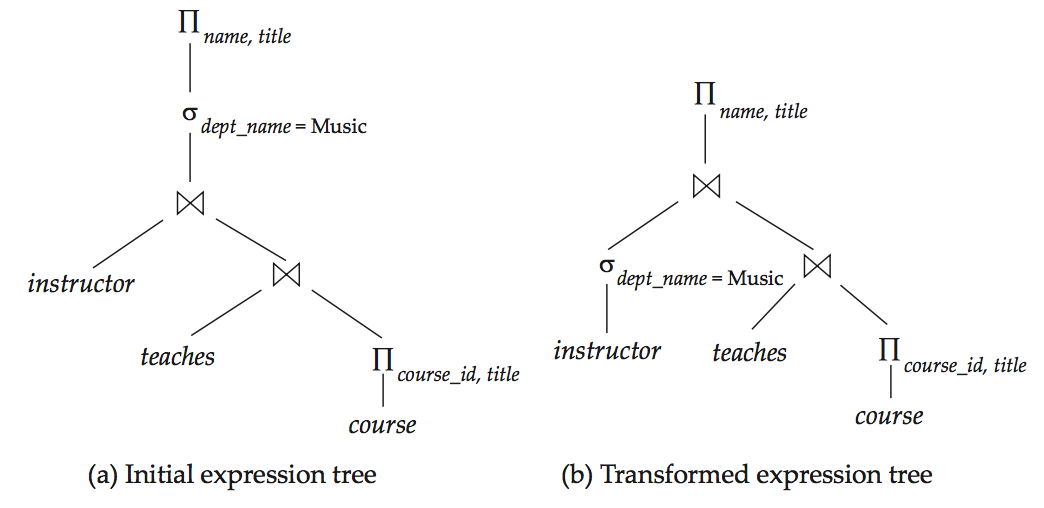
\includegraphics[width=0.7\textwidth]{images/optimization-1}
\end{center}

If it seems strange to you that the expressions can be rewritten a bit, it is more normal than one might expect. Compilers do this all the time, generating code that is equivalent to, but much faster than, the code that you wrote in the source file. If you would like to hear more about that, you could take ECE 459, Programming for Performance! 

This is only one possible transformation. Depending on the nature of the query, zero, one, or multiple equivalents may exist. It may be practical to write off some of those immediately, without assessing them, because we know they will be an inferior variant of a plan we have. The next step is then to draw up the plans for how we would execute the expressions. An annotated plan looks something like this~\cite{dsc}:

\begin{center}
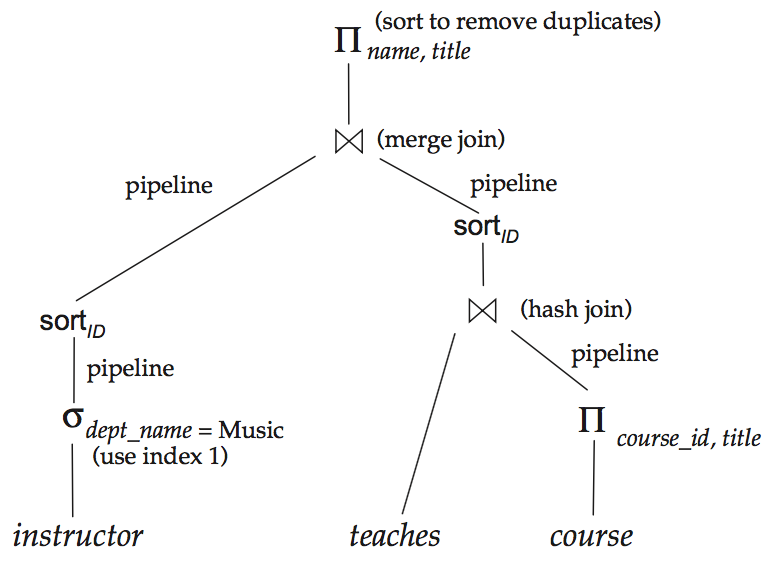
\includegraphics[width=0.45\textwidth]{images/optimization-2}
\end{center}

There may be many options for annotating each of the steps in the expression tree. A totally thorough approach would, once again, consider every possibility, but we realistically can eliminate some options that we know will be inferior to other choices. Then we may affix cost estimates to each plan as the sum of each part. The estimates can be wrong (it's why they are called estimates) but generally we can be sure we are at least in the correct ballpark. The final step is then to choose the the plan with the lowest cost. That last step is probably the least interesting since it just requires us to, well, compare some numbers and choose the smallest one.

As a practical note, in SQL you may ask the database server to tell you how it would carry out a query. First you write the query as you normally would and prefix this query with the keyword \texttt{EXPLAIN}\footnote{Every time I do this, I can't help but feel like this: \url{http://imgur.com/lUIlU4l}. I think the all-caps nature of the keyword contributes.}.

\subsection*{Expression Transformation}

There are some rules for how exactly to transform a query to an equivalent alternative. These are a little bit like some things you may have learned in mathematics, like how multiplication commutes or that addition is associative or something like that. There is probably nothing really saved by re-ordering a simple math expression like $12 \times 2 \times 3$, although you may find it personally faster or easier to do the math in your head by first computing $2 \times 3$ and multiplying the result by $12$ rather than first computing $12 \times 2$ and then multiplying it by $3$. Or you may personally find it easier to do the opposite, or have no preference whatsoever. But the idea applies.

We should remember that database operations do not, unless there is an explicit order-by clause, specify an order in which tuples appear in the output. Order does not matter in the output. If a request is for addresses where the province is ``ON'' or the province is ``QC'' then one execution plan may result in all tuples where province is ``ON'' followed by all provinces where the province is ``QC'' or the reverse, or they may be all mixed together. All three of those outcomes are equivalent as long as the same tuples are in the output.

There are some rules from~\cite{dsc} and~\cite{fds} that we want to learn about. To spare a lot of repetition of what things mean, the notation will be centralized here. $\theta_{x}$ denotes a predicate (as part of a selection or join, for example), $L_{x}$ denotes lists of attributes, and $E$ denotes a relational algebra expression (a sub-expression or a relation $r$). All our other symbols from relational algebra remain the same as when they were first introduced.

\paragraph{Rule 1: Conjunctive Selection}
Conjunctive selection can be turned into a sequence of individual selections. This makes sense: if we have a selection from address where province is ``ON'' and city is ``Kitchener'', we can do this as a selection on address where city is ``Kitchener'', producing a temporary relation and then we do a selection where province is ``ON'' on that temporary relation. That is sometimes called a cascade of selection.

In relational algebra: $\sigma_{\theta_{1} \wedge \theta_{2}}(E) = \sigma_{\theta_{1}}(\sigma_{\theta_{2}}(E))$


\paragraph{Rule 2: Selection Commutes}
Selection commutes. Suppose the original selection is on address where city is ``Kitchener'', producing a temporary relation and then we do a selection where province is ``ON'' on that temporary relation. This is equivalent to doing a selection on address where province is ``ON'' and producing a temporary relation, and then we can select where city is ``Kitchener'' on the temporary relation. The results are identical in both cases. 

In relational algebra: $\sigma_{\theta_{1}}(\sigma_{\theta_{2}}(E)) = \sigma_{\theta_{2}}(\sigma_{\theta_{1}}(E))$

\paragraph{Rule 3: Projection Redundancy Elimination}

Only the last projection operation is needed; all other projection operations do not do anything. This should be pretty logical given that projection reduces the returned attributes to just those that are specified in the projection.

In relational algebra: $\Pi_{L_{1}}(\Pi_{L_{2}}(\Pi_{L_{3}}(E))) = \Pi_{L_{1}}(E)$

\paragraph{Rule 4: Commuting Selection and Projection}
If a selection involves the same attributes as a projection list, we can commute the two operations. That is, if $L$ contains exactly the same set of attributes $A_{1}, A_{2}...$ that are referenced in $\theta$ then:

$\Pi_{L}(\sigma_{\theta}(E)) = \sigma_{\theta}(\Pi_{L}(E))$

\paragraph{Rule 5: Selection Combination}

Selection may be combined with both cartesian product. This is, as you will recall, how a theta join works and is shown as (a) below in the relational algebra. If a selection being combined with what is already a theta join, that is the same as a theta join with a conjunctive predicate, shown as (b) below in relational algebra.

a. $\sigma_{\theta}(E_{1} \times E_{2}) = E_{1} \bowtie_{\theta} E_{2}$

b. $\sigma_{\theta_{1}}( E_{1} \bowtie_{\theta_{2}} E_{2}) = E_{1} \bowtie_{\theta_{1}\wedge\theta_{2}} E_{2}$

\paragraph{Rule 6: Theta Joins Commute}
Theta (and natural) joins commute, so the operands can be swapped in order and the same result is produced. That is a relief, considering our previous discussion of what blocks need to get moved into memory to complete the operation. This does potentially change the order of the attributes in the output, but we should not actually care. Normally a selection statement, for example, specifies some attributes to be returned, meaning there is a projection operation to be done. If there is a select \texttt{*} operation, no order is guaranteed in the output anyway.

In relational algebra: $E_{1} \bowtie_{\theta} E_{2} = E_{2} \bowtie_{\theta} E_{1}$

The natural join is a special case of the theta join, so $E_{1} \bowtie E_{2} = E_{2} \bowtie E_{1}$

\paragraph{Rule 7: Natural Join Associates}
When discussing joins, we actually already covered this rule, that they are associative, i.e. we can do them pairwise in whichever order we prefer. For theta joins, it looks a little more complicated, but the outcome is the same, keeping in mind that $\theta_{2}$ references only attributes of Expressions 2 and 3 (so it can't really be applied to Expression 1).


a. $(E_{1} \bowtie E_{2}) \bowtie E_{3} = E_{1} \bowtie (E_{2} \bowtie E_{3})$. 

b. $(E_{1} \bowtie_{\theta_{1}} E_{2}) \bowtie_{\theta_{2}\wedge\theta_{3}} E_{3} = E_{1} \bowtie_{\theta_{1}\wedge\theta_{3}} (E_{2} \bowtie_{\theta_{2}} E_{3})$. 

c. Because cartesian product is an empty theta join, $(E_{1} \times E_{2}) \times E_{3} = E_{1} \times (E_{2} \times E_{3})$. 


\paragraph{Rule 8: Selection Distribution}
Selection distributes over theta join if the following conditions hold:

a. It distributes if all the attributes in $\theta_{0}$ involve only the attributes of one of the expressions $E$ being joined. This means we can cut down the first relation to only the matching rows before performing the join, which is hopefully a faster way to do it. In this example, if $\theta_{0}$ applies only to $E_{1}$:

$\sigma_{\theta_{0}}(E_{1} \bowtie_{\theta} E_{2}) = (\sigma_{\theta_{0}}(E_{1})) \bowtie_{\theta} E_{2}$ 

b. It distributes when $\theta_{1}$ involves only the attributes of $E_{1}$ and $\theta_{2}$ only the attributes of $E_{2}$. This would mean cutting down both relations before performing the join.

$\sigma_{\theta_{1}\wedge\theta_{2}} (E_{1} \bowtie_{\theta} E_{2}) = (\sigma_{\theta_{1}}(E_{1})) \bowtie_{\theta} (\sigma_{\theta_{2}}(E_{2})) $

Both of these scenarios apply also for the cartesian product.

\paragraph{Rule 9: Projection Distribution}
The projection operation can be distributed over theta join if the following conditions hold:

a. If $L_{1}$ and $L_{2}$ are attributes of $E_{1}$ and $E_{2}$ respectively, and $\theta$ contains only attributes in $L_{1} \cup L_{2}$, then we can distribute. This means that we can, much like the previous rule, cut down the relations using the projection before performing the join:

$\Pi_{L_{1} \cup L_{2}}( E_{1} \bowtie_{\theta} E_{2} ) = (\Pi_{L_{1}}(E_{1})) \bowtie_{\theta} (\Pi_{L_{2}}(E_{2}))$

b. If $L_{1}$ and $L_{2}$ are attributes of $E_{1}$ and $E_{2}$ respectively, and $L_{3}$ are join attributes of $E_{1}$ not $L_{1} \cup L_{2}$ and $L_{4}$ are join attributes of $E_{2}$ not $L_{1} \cup L_{2}$:

$\Pi_{L_{1} \cup L_{2}} (E_{1} \bowtie_{\theta} E_{2}) = \Pi_{L_{1} \cup L_{2}}((\Pi_{L_{1} \cup L_{3}}(E1)) \bowtie_{\theta} (\Pi_{L_{2} \cup L_{4}}(E_{2})))$

Again, this can also be applied to cartesian product.

\paragraph{Rule 10: Set Operations Commute}

The set operations union and intersection commute  (difference does not).

a. $E_{1} \cup E_{2} = E_{2} \cup E_{1}$

b. $E_{1} \cap E_{2} = E_{2} \cap E_{1}$

\paragraph{Rule 11: Set Operations Associate}
Union and intersection are associative:

a. $(E_{1} \cup E_{2}) \cup E_{3} = E_{1} \cup (E_{2} \cup E_{3})$

b. $(E_{1} \cap E_{2}) \cap E_{3} = E_{1} \cap (E_{2} \cap E_{3})$

\paragraph{Rule 12: Selection Distribution II}

Selection distributes over union, intersection, and difference operations:

a. $\sigma_{\theta}(E_{1} \cup E_{2}) = \sigma_{\theta}(E_{1}) \cup \sigma_{\theta}(E_{2})$

b. $\sigma_{\theta}(E_{1} \cap E_{2}) = \sigma_{\theta}(E_{1}) \cap \sigma_{\theta}(E_{2})$

c. $\sigma_{\theta}(E_{1} - E_{2}) = \sigma_{\theta}(E_{1}) - \sigma_{\theta}(E_{2})$

\paragraph{Rule 13: Projection Distribution II}
The projection operation distributes over a union operation.

In relational algebra: $\Pi_{L}(E_{1} \cup E_{2} = (\Pi_{L}(E_{1}))\cup(\Pi_{L}(E_{2}))$

\subsubsection*{Rules Review}

These rules are (sadly) neither a complete set nor minimal. There are other potential transformations that can be done, including various rules from boolean algebra (e.g., $\neg (a \wedge b) = \neg a \vee \neg b$) that are not covered here~\cite{fds}. As we might see from looking at the rules as well, it is possible to use certain rules to derive other ones in that list. This is okay, as they are intended as a human comprehensible list. If we were actually writing these for the computer we would probably want a minimal set to reduce the amount of computation done to generate all the equivalent transformations. 

Having learned a bit about equivalence rules and what they are for, next time we will work on putting them to use and affixing cost estimates.

\bibliographystyle{alphaurl}
\bibliography{356}


\end{document}
